\section{Planteamiento del Problema} \label{problem_statement}

La empresa de prefabricados ArenA, en su interés por ampliar el catálogo de productos, enfrenta una problemática inicial relacionada con la falta de un sistema efectivo para controlar los inventarios de producción, calcular los costos de producción de manera continua y obtener información relevante, histórica y sintetizada. Este vacío dificulta la toma de decisiones basadas en datos objetivos y la consecuente planificación del uso de materiales, generando ineficacias en la gestión de recursos y probablemente afectando la rentabilidad de la empresa.

En un esfuerzo por resolver esta situación, se intentó implementar sistemas ERP convencionales. Sin embargo, aunque estos sistemas ofrecen funcionalidades completas y versátiles, su complejidad y necesidad de configurar múltiples módulos para escenarios diversos los convierten en herramientas poco prácticas para la empresa. Este problema se agrava considerando que el personal encargado de su uso, en parte, no cuenta con formación académica avanzada, aunque tiene experiencia utilizando dispositivos móviles. También es de notar que los costos de dichas herramientas crecen de forma proporcional al número de usuarios con un pago en dólares que podría ascender facilmente por encima de los 1000 dólares americanos para tan sólo 5 usuarios \cite{martinCleanCodeHandbook2009}.

\begin{figure}[htbp]
    \centering
    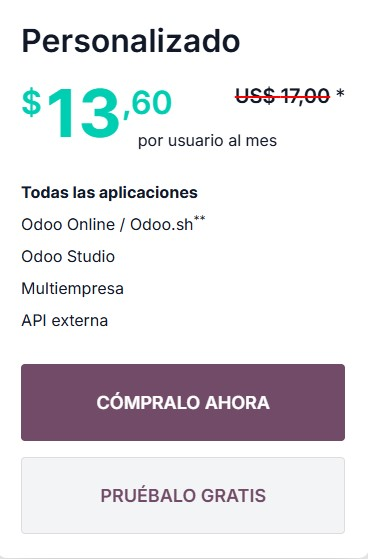
\includegraphics[width=0.3\textwidth]{assets/oddopricing.JPG}
    \caption{Costo mensual por usuario de un ERP popular}
    \label{fig:oddopricing}
\end{figure}


Además, los procesos productivos de la empresa presentan características específicas que no son plenamente compatibles con los flujos estándar de un ERP tradicional. Esto genera un sobredimensionamiento del sistema, con funcionalidades innecesarias que no solo complican su uso, sino que también incrementan los costos de implementación, capacitación y mantenimiento.

Por otro lado, la empresa no requiere la gama completa de funciones que un ERP ofrece. Su necesidad se centra en las actividades de planeación de materiales y recursos (MRP) propias de su modelo de producción, como la gestión de inventarios, la programación de pedidos y el control de recursos para cumplir con los tiempos de entrega. Sin embargo, las soluciones actuales no ofrecen un equilibrio adecuado entre simplicidad, accesibilidad y personalización, dejando un vacío importante en su capacidad operativa.

Esto plantea la necesidad de desarrollar una solución de software específica que no solo atienda la problemática original del control de inventarios y cálculo continuo de costos de producción, sino que también sea accesible para usuarios sin formación técnica avanzada y optimice los procesos productivos sin introducir complejidad innecesaria. Un sistema diseñado a medida puede resolver estas problemáticas al enfocarse exclusivamente en las funcionalidades necesarias y al ofrecer una interfaz amigable y adecuada para el perfil de los usuarios finales.
